% CREATED BY DAVID FRISK, 2016
\chapter{Accelerator library}

\definecolor{commentsColor}{rgb}{0.497495, 0.497587, 0.497464}
\definecolor{keywordsColor}{rgb}{0.000000, 0.000000, 0.635294}
\definecolor{stringColor}{rgb}{0.558215, 0.000000, 0.135316}


\definecolor{vgreen}{RGB}{104,180,104}
\definecolor{vblue}{RGB}{49,49,255}
\definecolor{vorange}{RGB}{255,143,102}

Script for creating library:
\lstinputlisting[  backgroundcolor=\color{white},   % choose the background color; you must add \usepackage{color} or \usepackage{xcolor}
  basicstyle=\footnotesize,        % the size of the fonts that are used for the code
  breakatwhitespace=false,         % sets if automatic breaks should only happen at whitespace
  breaklines=true,                 % sets automatic line breaking
  captionpos=b,                    % sets the caption-position to bottom
  commentstyle=\color{commentsColor}\textit,    % comment style
  deletekeywords={...},            % if you want to delete keywords from the given language
  escapeinside={\%*}{*)},          % if you want to add LaTeX within your code
  extendedchars=true,              % lets you use non-ASCII characters; for 8-bits encodings only, does not work with UTF-8
%  frame=tb,	                   	   % adds a frame around the code
  keepspaces=true,                 % keeps spaces in text, useful for keeping indentation of code (possibly needs columns=flexible)
  keywordstyle=\color{keywordsColor}\bfseries,       % keyword style
  language=Python,                 % the language of the code (can be overrided per snippet)
  otherkeywords={*,...},           % if you want to add more keywords to the set
  numbers=left,                    % where to put the line-numbers; possible values are (none, left, right)
  numbersep=5pt,                   % how far the line-numbers are from the code
  numberstyle=\tiny\color{commentsColor}, % the style that is used for the line-numbers
  rulecolor=\color{black},         % if not set, the frame-color may be changed on line-breaks within not-black text (e.g. comments (green here))
  showspaces=false,                % show spaces everywhere adding particular underscores; it overrides 'showstringspaces'
  showstringspaces=false,          % underline spaces within strings only
  showtabs=false,                  % show tabs within strings adding particular underscores
  stepnumber=1,                    % the step between two line-numbers. If it's 1, each line will be numbered
  stringstyle=\color{stringColor}, % string literal style
  tabsize=2,	                   % sets default tabsize to 2 spaces
%  title=\lstname,                  % show the filename of files included with \lstinputlisting; also try caption instead of title
  columns=fixed                    % Using fixed column width (for e.g. nice alignment)
firstline=1, lastline=59]{../../dtpu/software/create_library.py}
\newpage
C++ code of the library:
\lstinputlisting[language=C++]{../../dtpu/software/DTPU_delegate.cpp}
\newpage
Frozen python code in the accelerator library:
\lstinputlisting[language=Python]{../../dtpu/software/DTPU_delegate.py}

\chapter{Top level entity of DTPU core}

\lstinputlisting[style={verilog-style}]{../../dtpu/files/dtpu_core.v}

\chapter{Results for different frequencies}

\begin{figure}[!htbp]
\centering
\captionsetup{justification=centering}
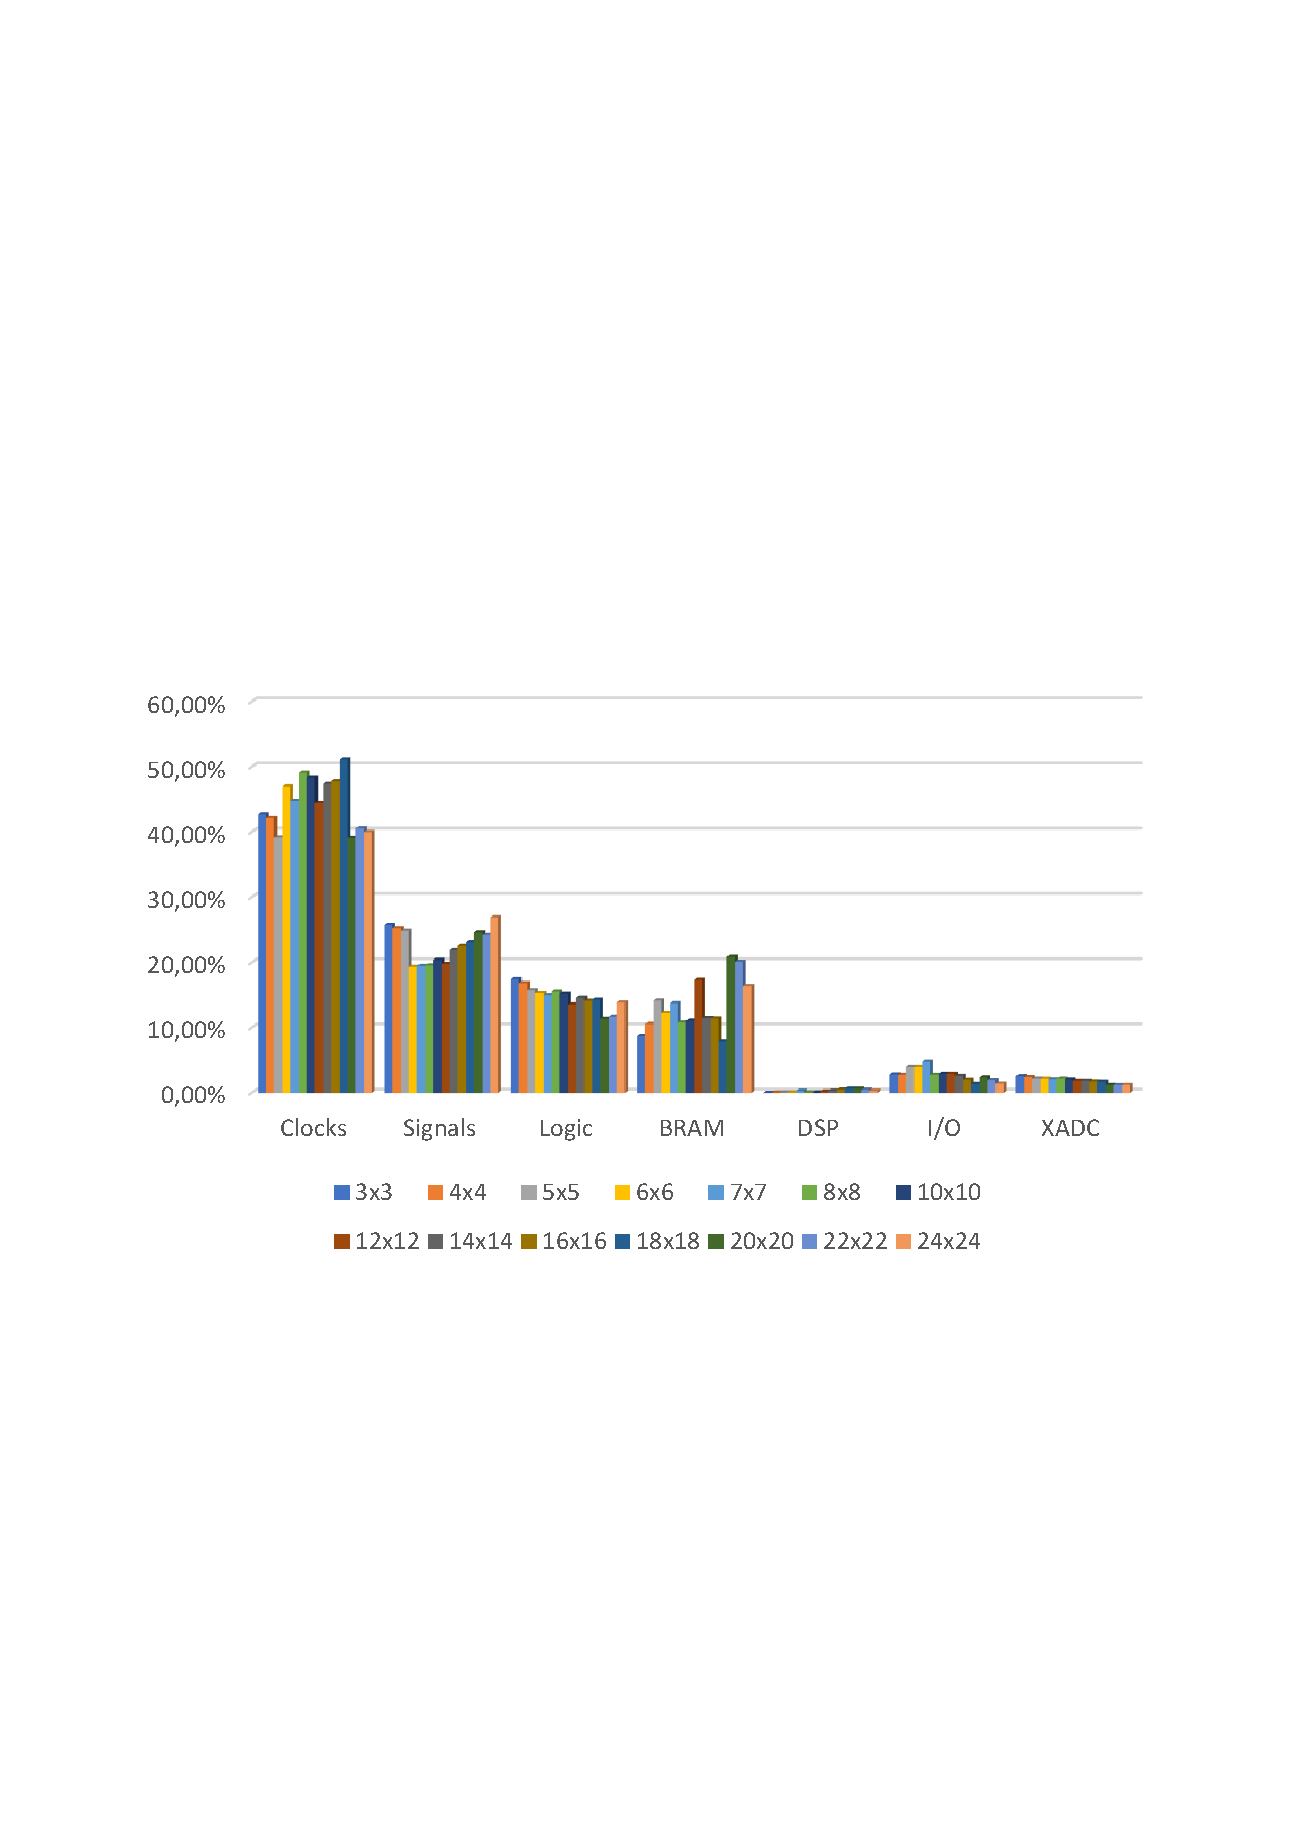
\includegraphics[scale=0.7,angle=0]{./figure/graphs/power_pldyn_div_int8_freq_50mhz.pdf}
\caption{Post Implementation Dynamic Power Consumption per entities in Programmable Logic with a clock frequency of 50 MHz and integer 8 PEs}
\label{fig:dynpowint8ent50}
\end{figure}
\begin{figure}[!htbp]
\centering
\captionsetup{justification=centering}
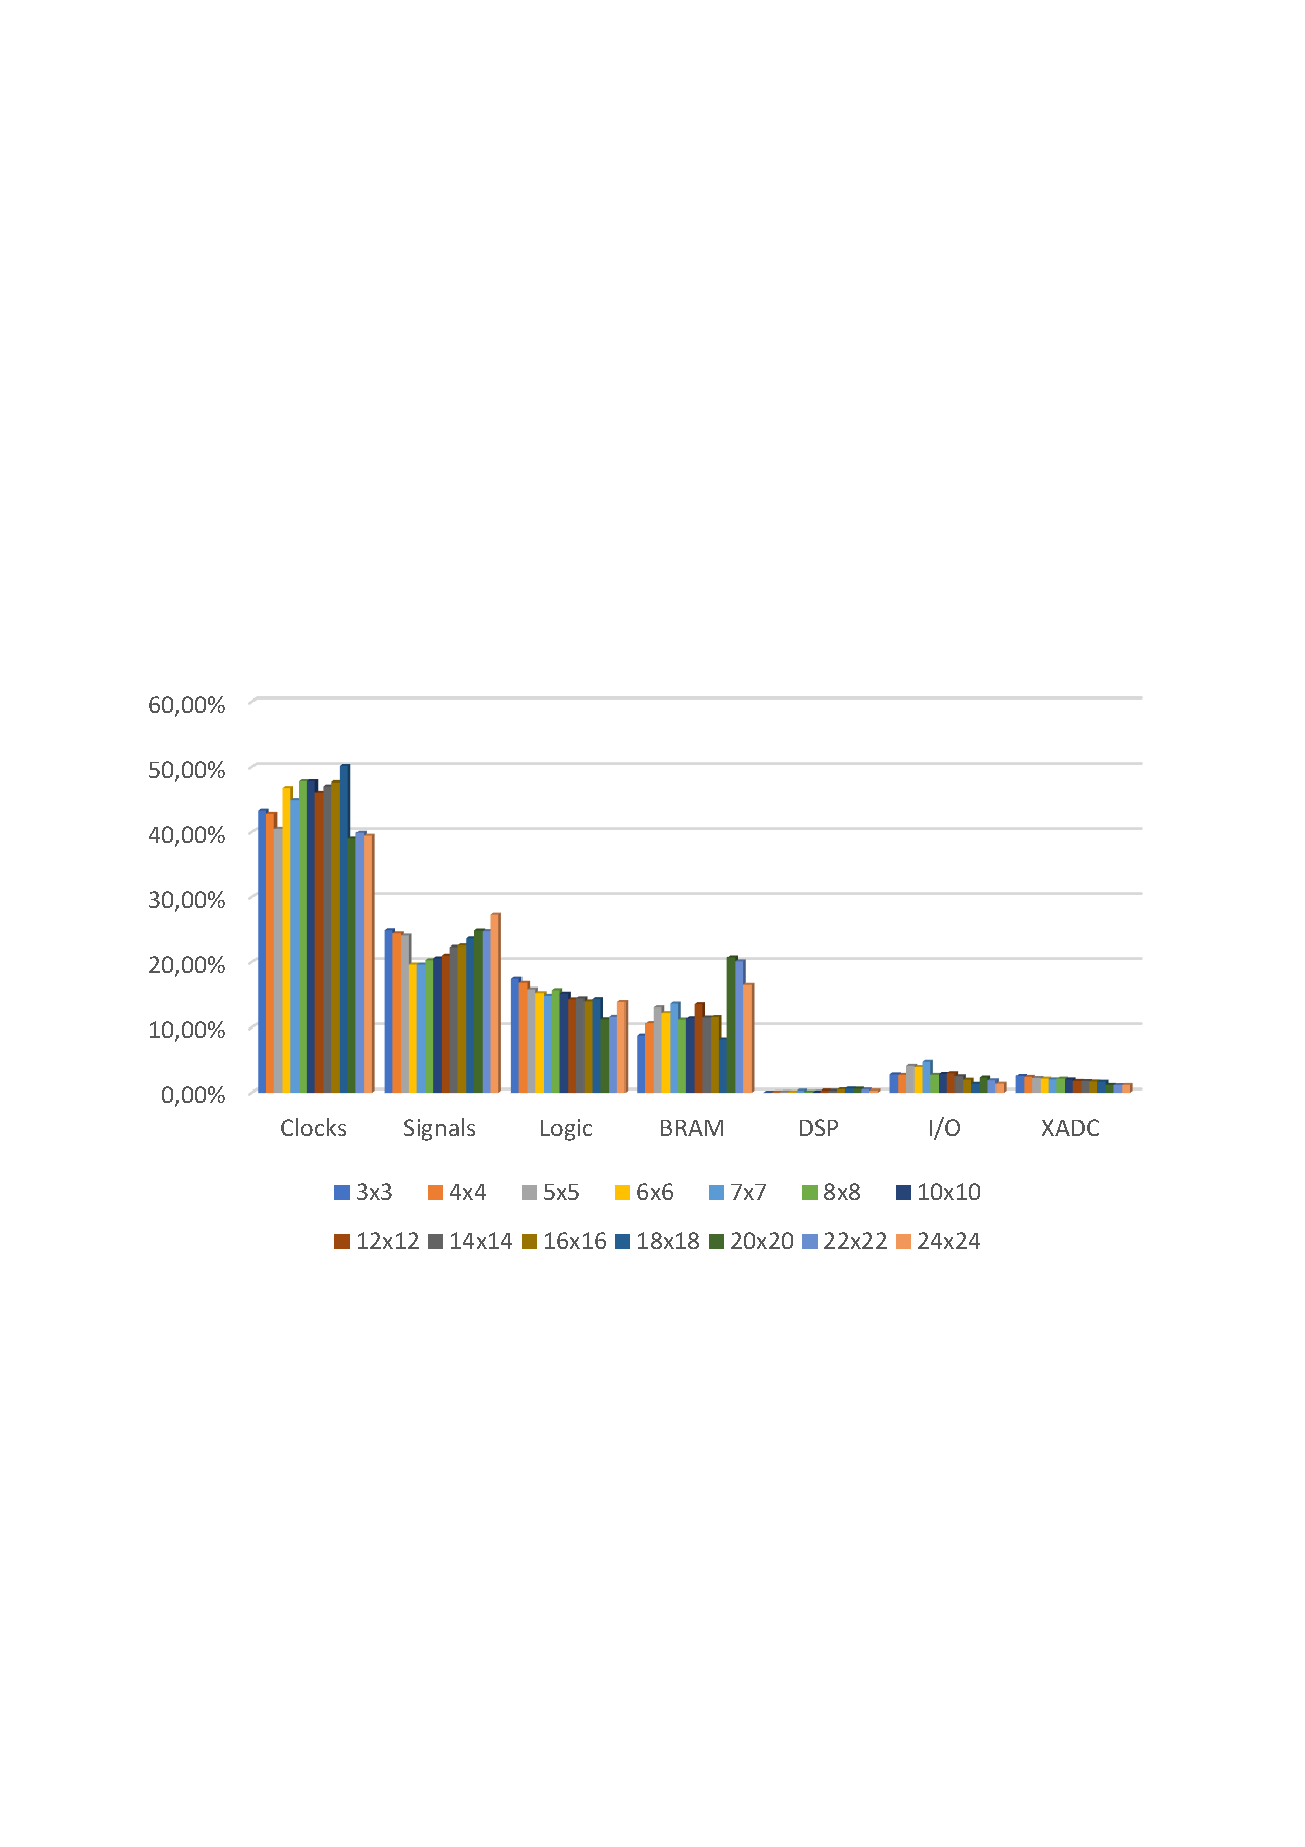
\includegraphics[scale=0.7,angle=0]{./figure/graphs/power_pldyn_div_int8_freq_80mhz.pdf}
\caption{Post Implementation Dynamic Power Consumption per entities in Programmable Logic with a clock frequency of 80 MHz and integer 8 PEs}
\label{fig:dynpowint8ent80}
\end{figure}
\begin{figure}[!htbp]
\centering
\captionsetup{justification=centering}
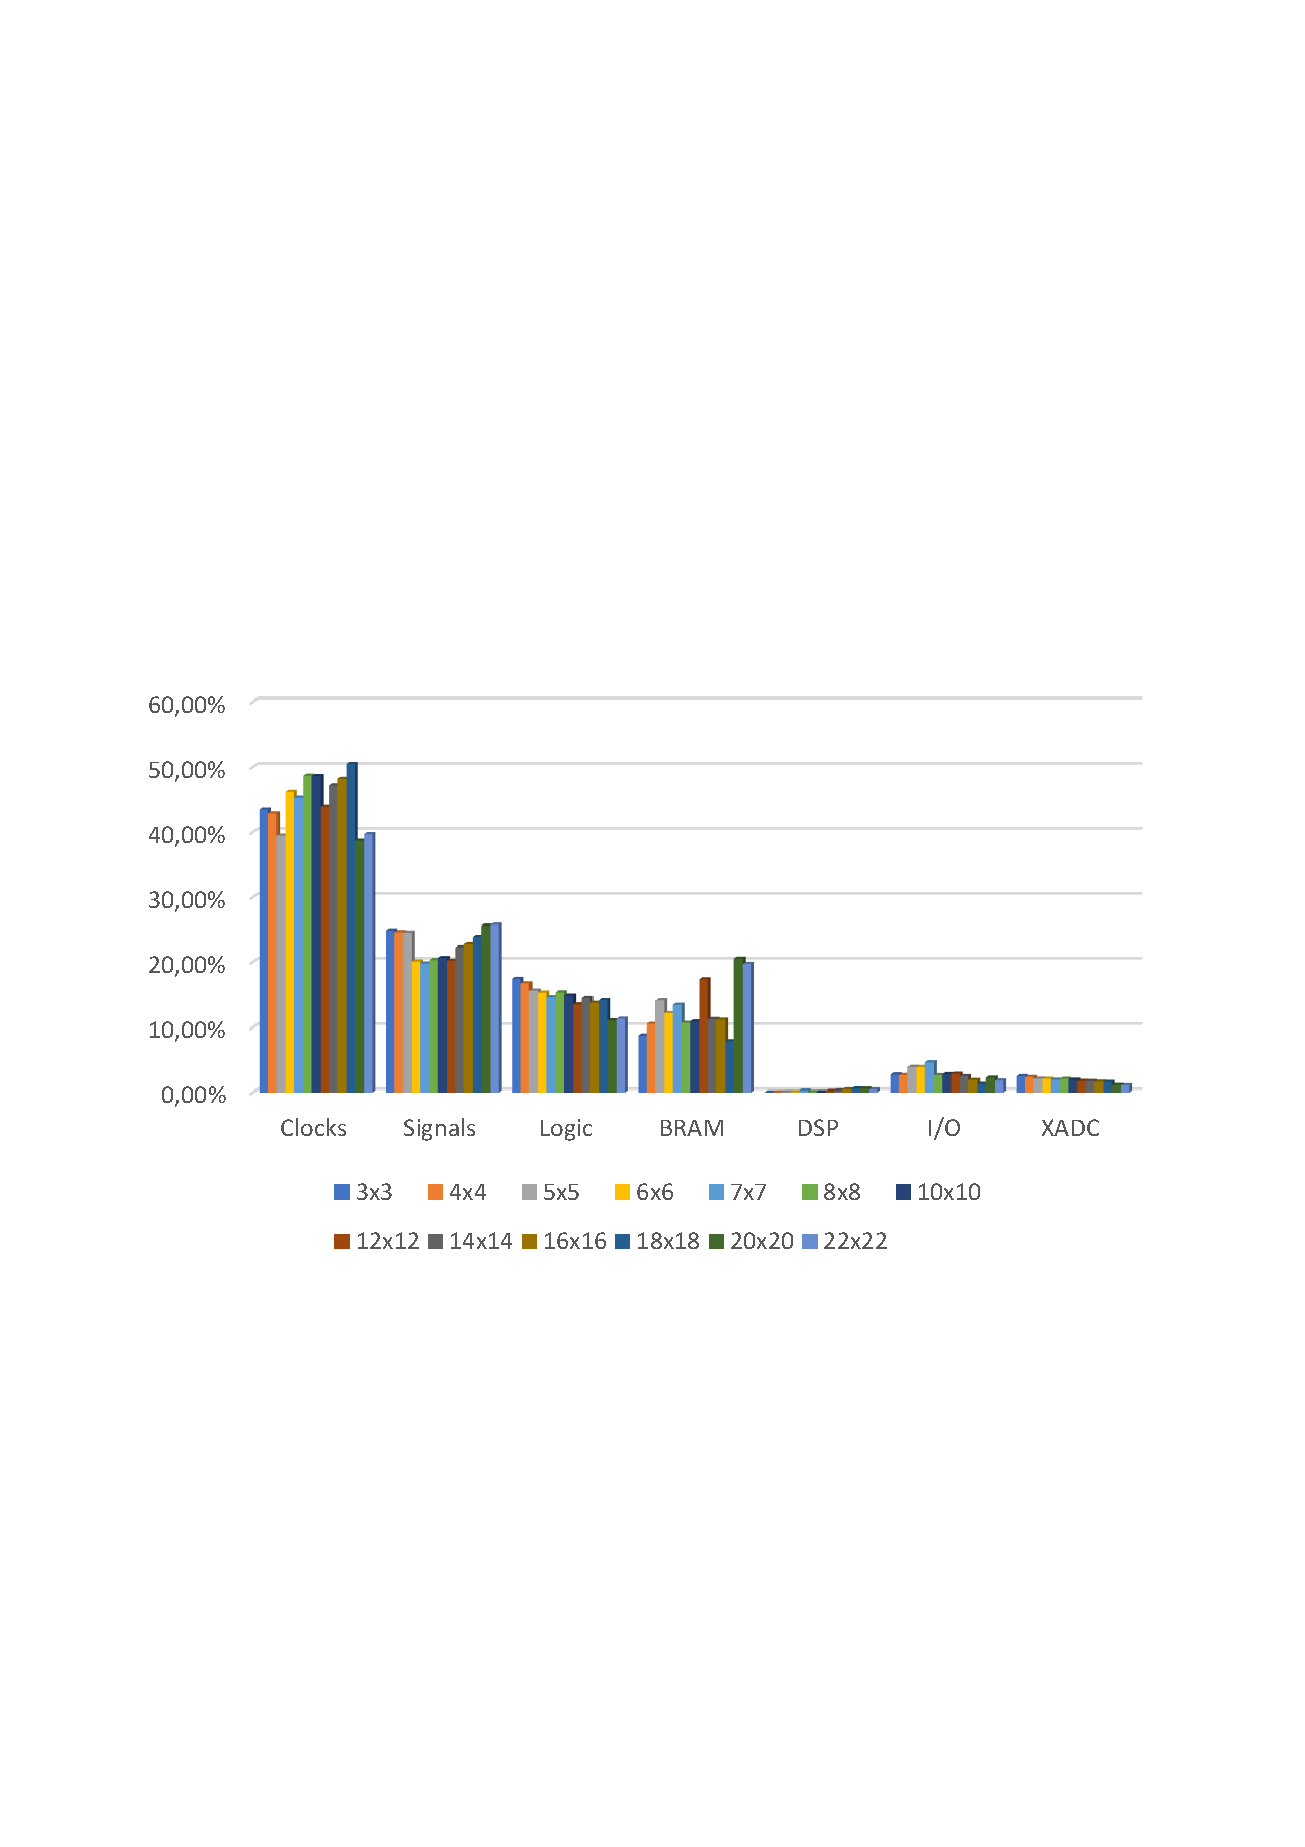
\includegraphics[scale=0.7,angle=0]{./figure/graphs/power_pldyn_div_int8_freq_100mhz.pdf}
\caption{Post Implementation Dynamic Power Consumption per entities in Programmable Logic with a clock frequency of 100 MHz and integer 8 PEs}
\label{fig:dynpowint8ent100}
\end{figure}
\begin{figure}[!htbp]
\centering
\captionsetup{justification=centering}
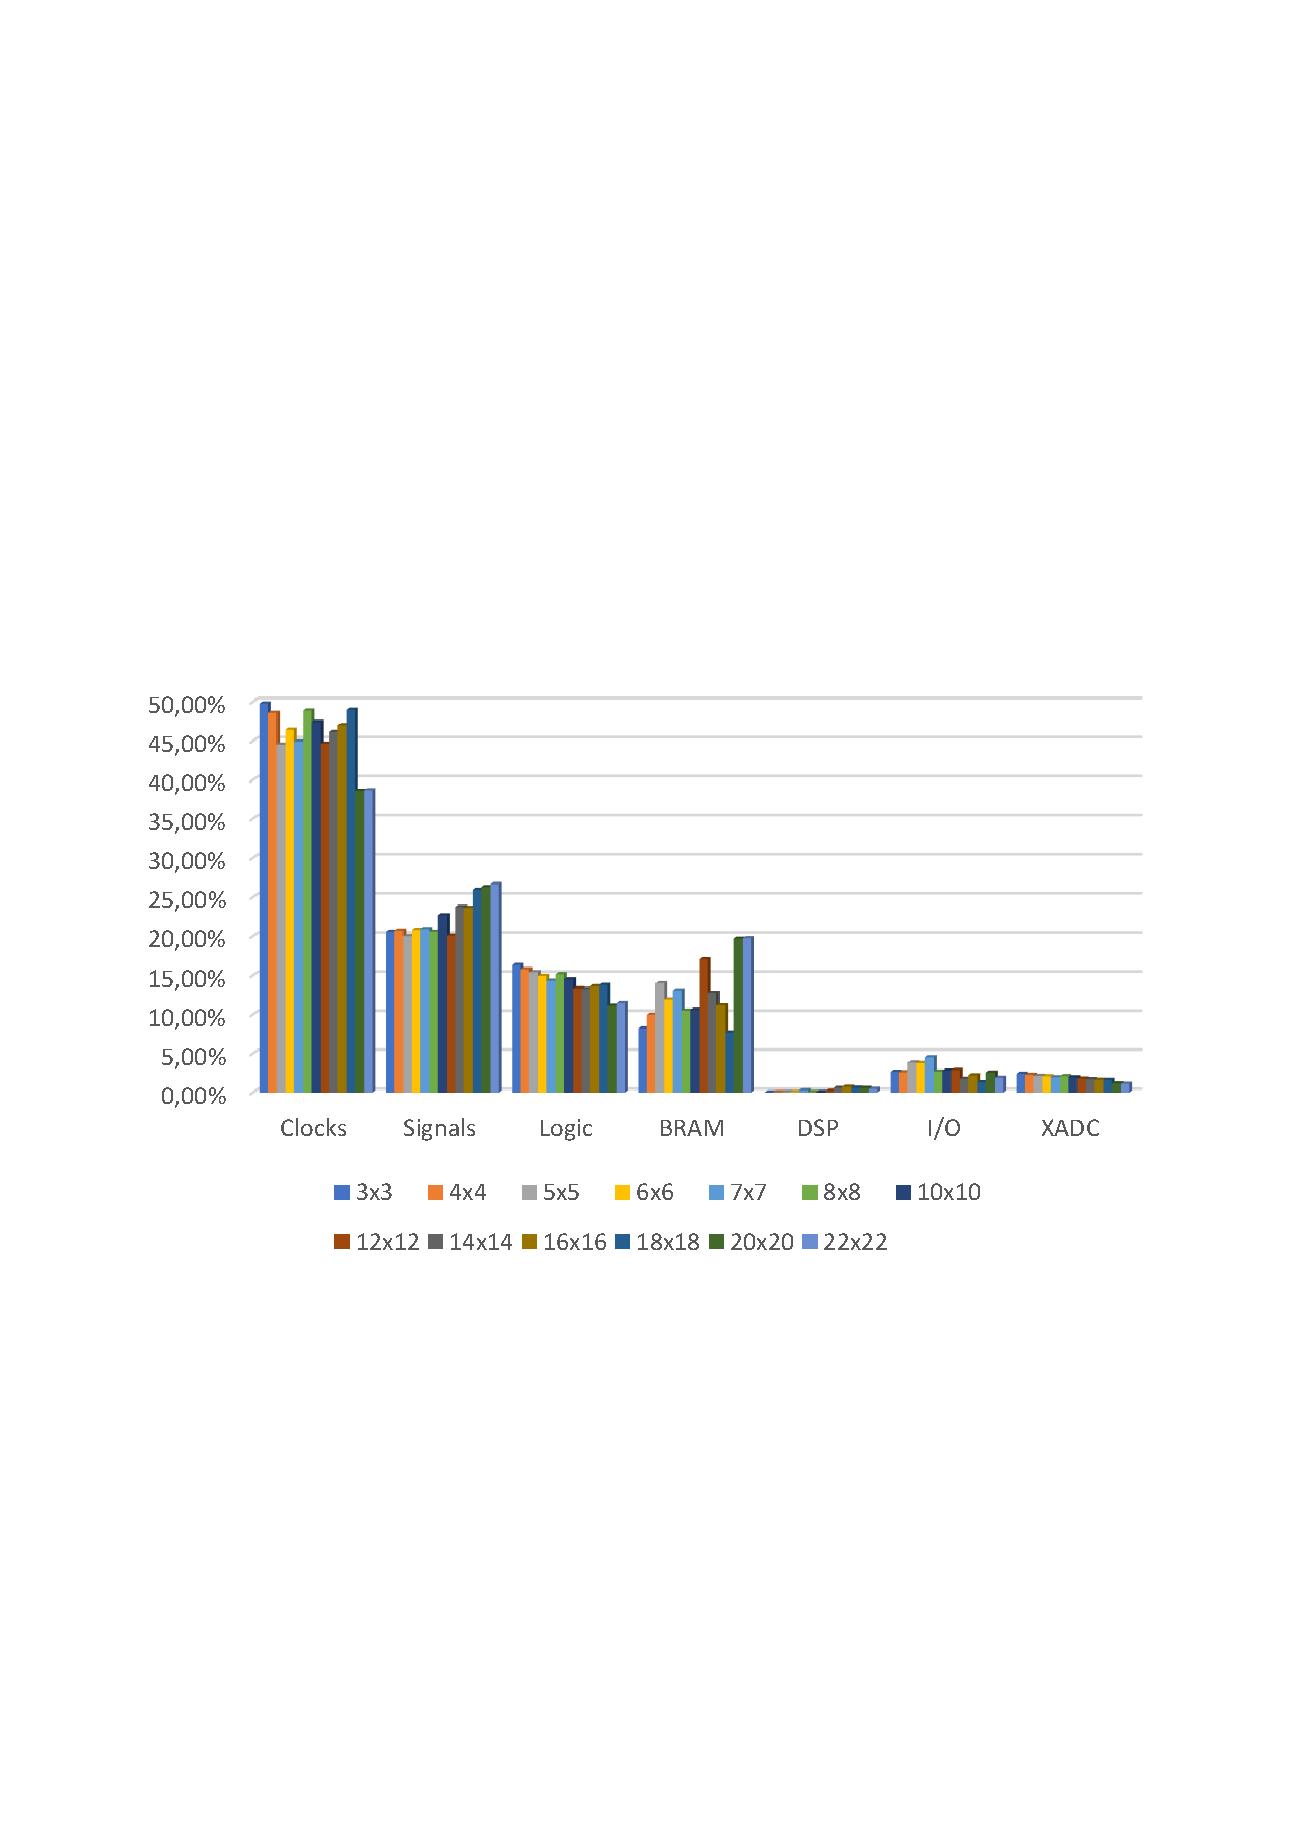
\includegraphics[scale=0.7,angle=0]{./figure/graphs/power_pldyn_div_int8_freq_120mhz.pdf}
\caption{Post Implementation Dynamic Power Consumption per entities in Programmable Logic with a clock frequency of 120 MHz and integer 8 PEs}
\label{fig:dynpowint8ent120}
\end{figure}

\begin{figure}[!htbp]
\centering
\captionsetup{justification=centering}
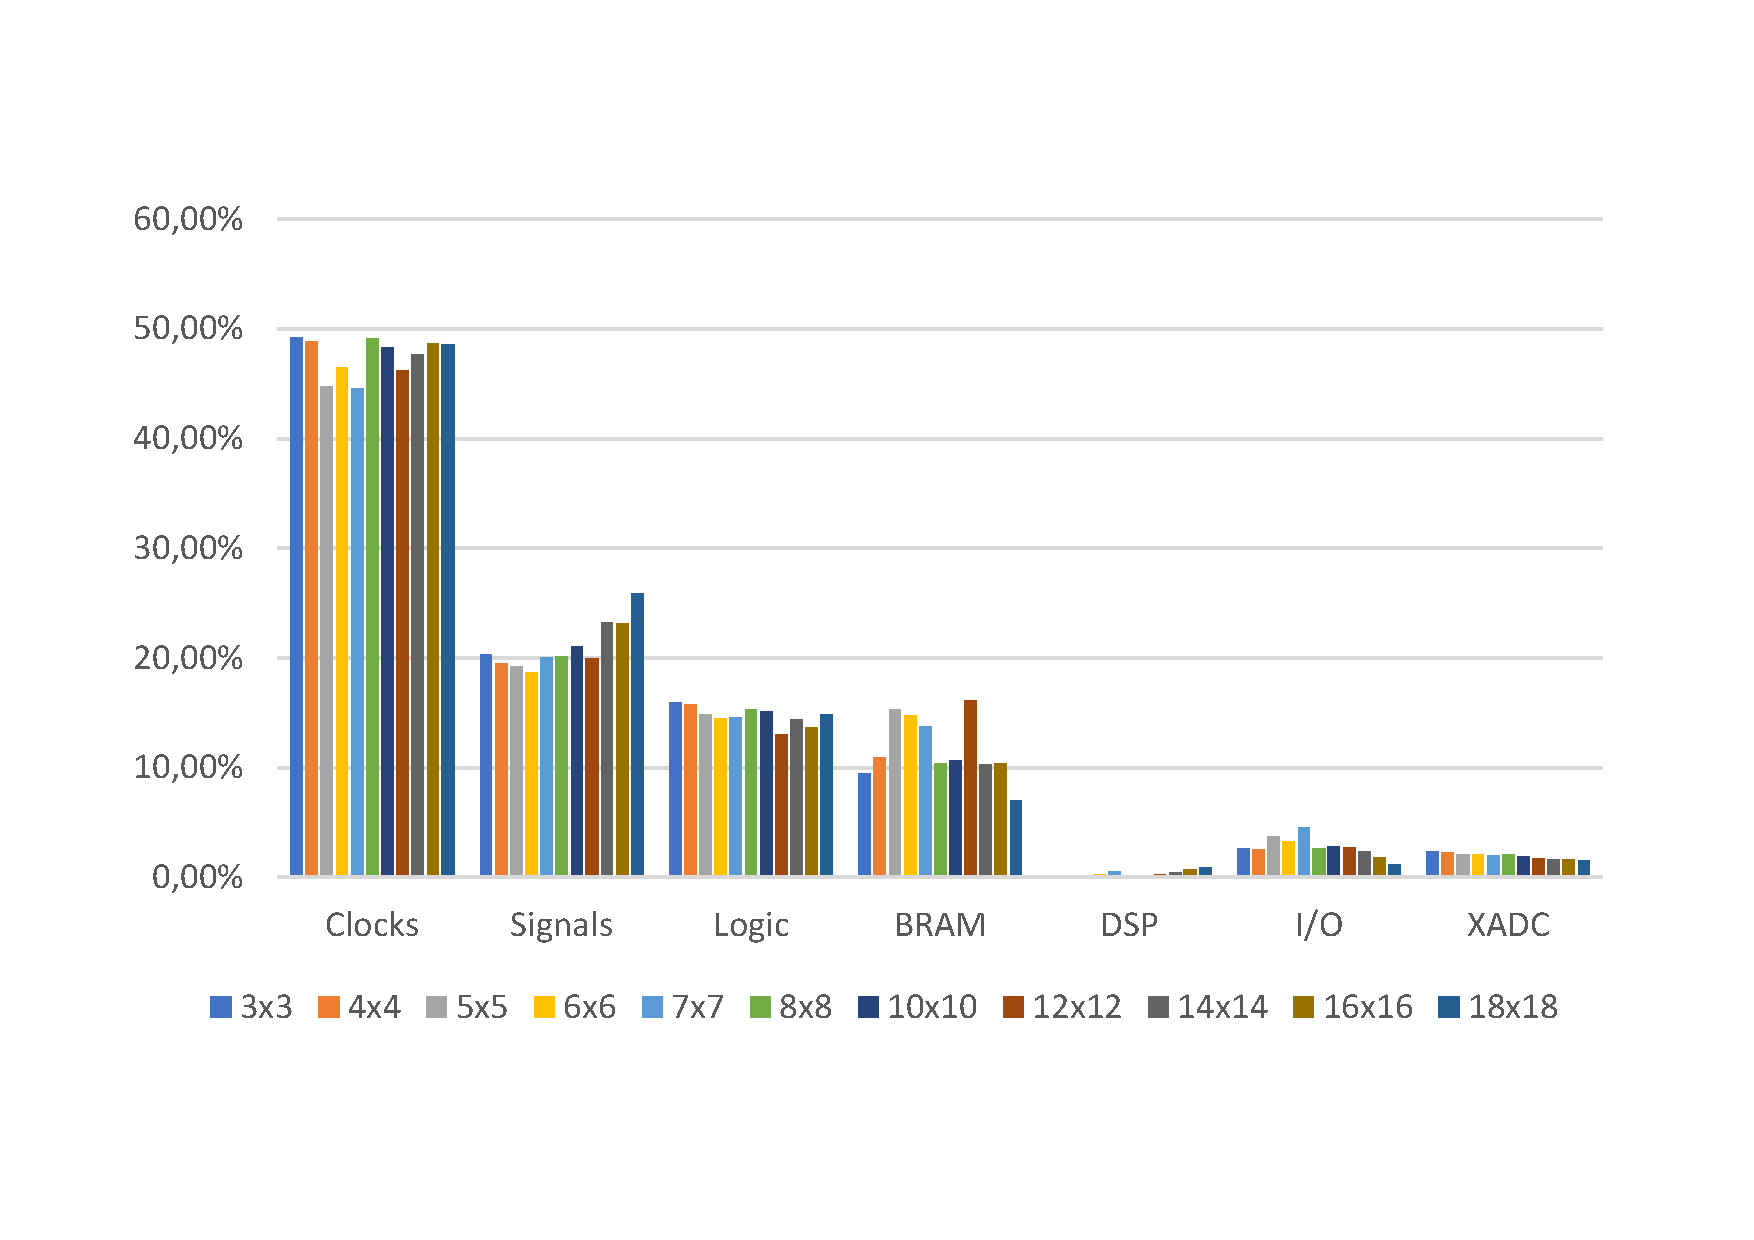
\includegraphics[scale=0.6,angle=0]{./figure/graphs/power_pldyn_div_int16_freq_50mhz.pdf}
\caption{Post Implementation Dynamic Power Consumption per entities in Programmable Logic with a clock frequency of 50 MHz and integer 16 PEs}
\label{fig:dynpowint16ent50}
\end{figure}
\begin{figure}[!htbp]
\centering
\captionsetup{justification=centering}
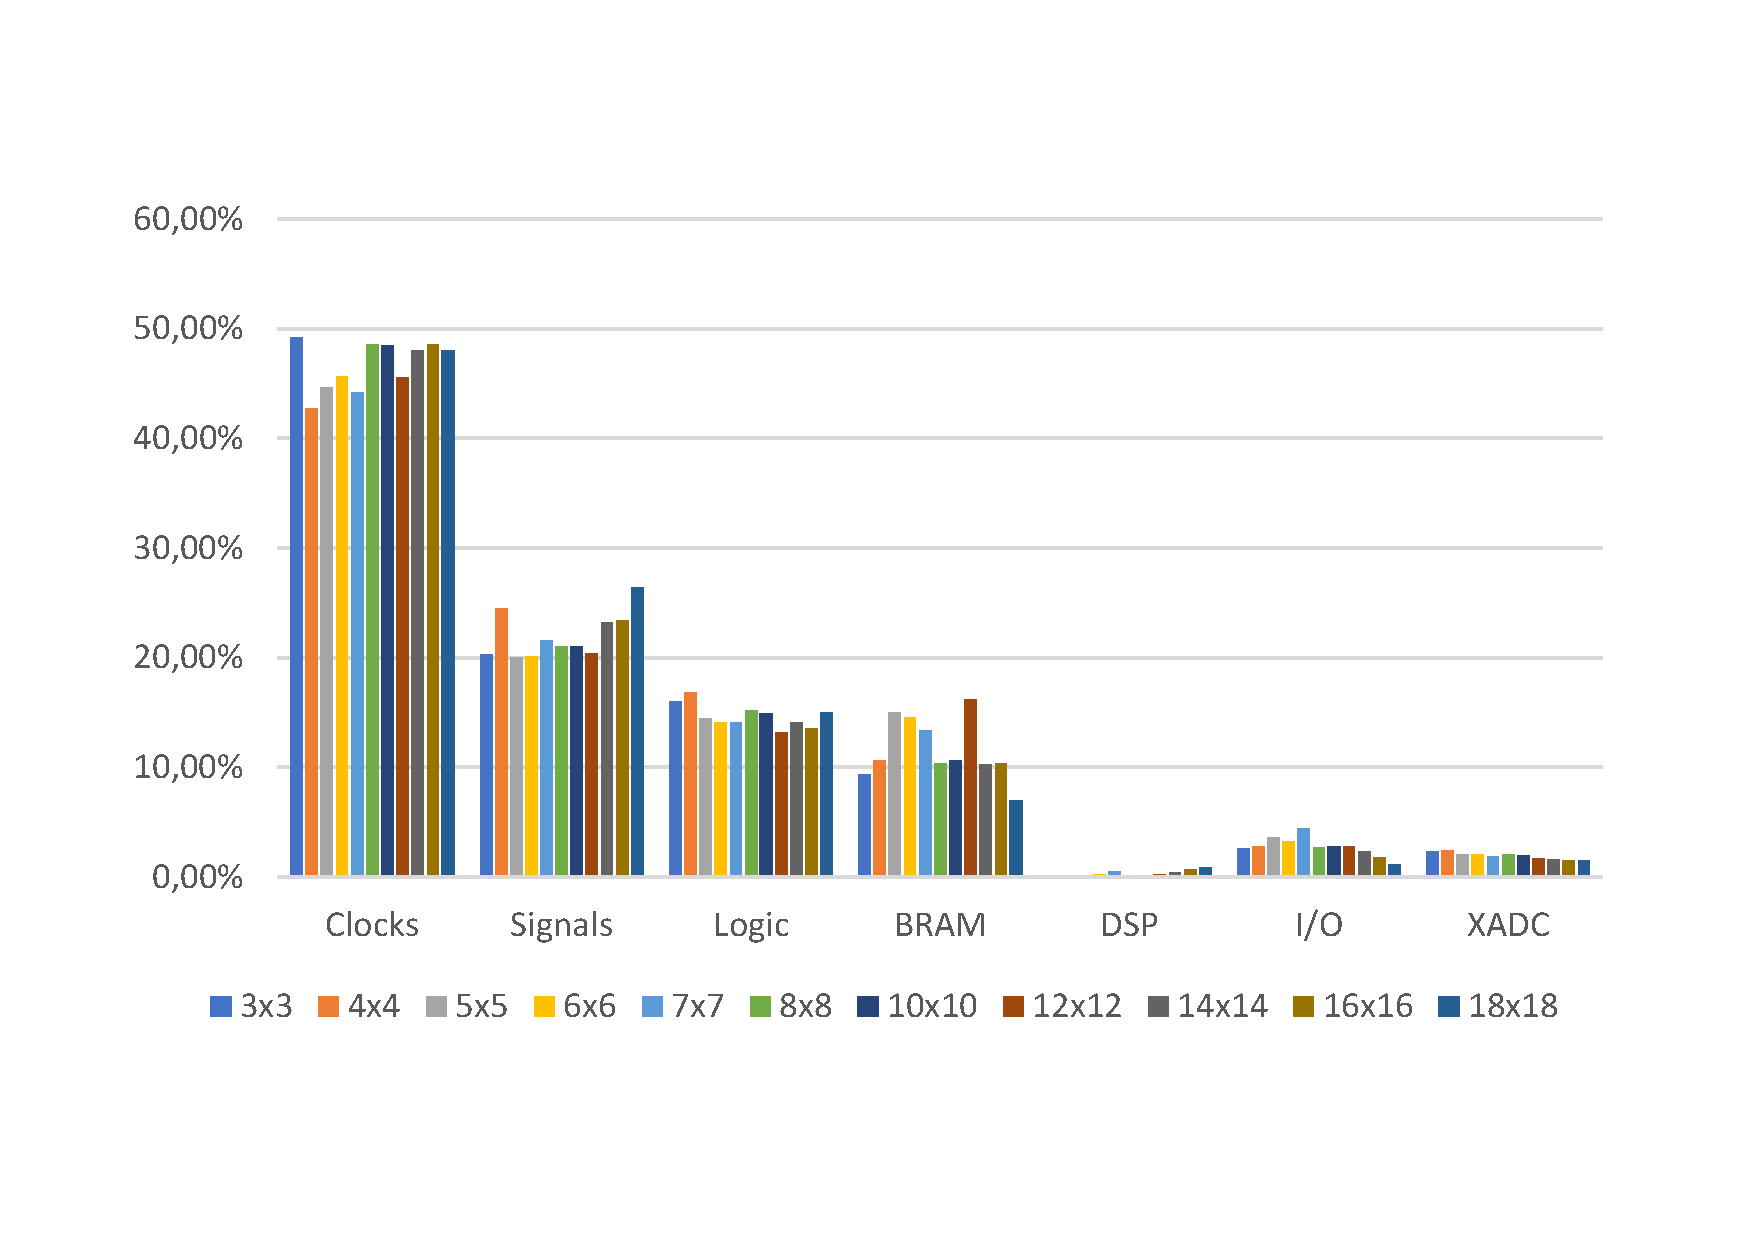
\includegraphics[scale=0.6,angle=0]{./figure/graphs/power_pldyn_div_int16_freq_80mhz.pdf}
\caption{Post Implementation Dynamic Power Consumption per entities in Programmable Logic with a clock frequency of 80 MHz and integer 16 PEs}
\label{fig:dynpowint16ent80}
\end{figure}
\begin{figure}[!htbp]
\centering
\captionsetup{justification=centering}
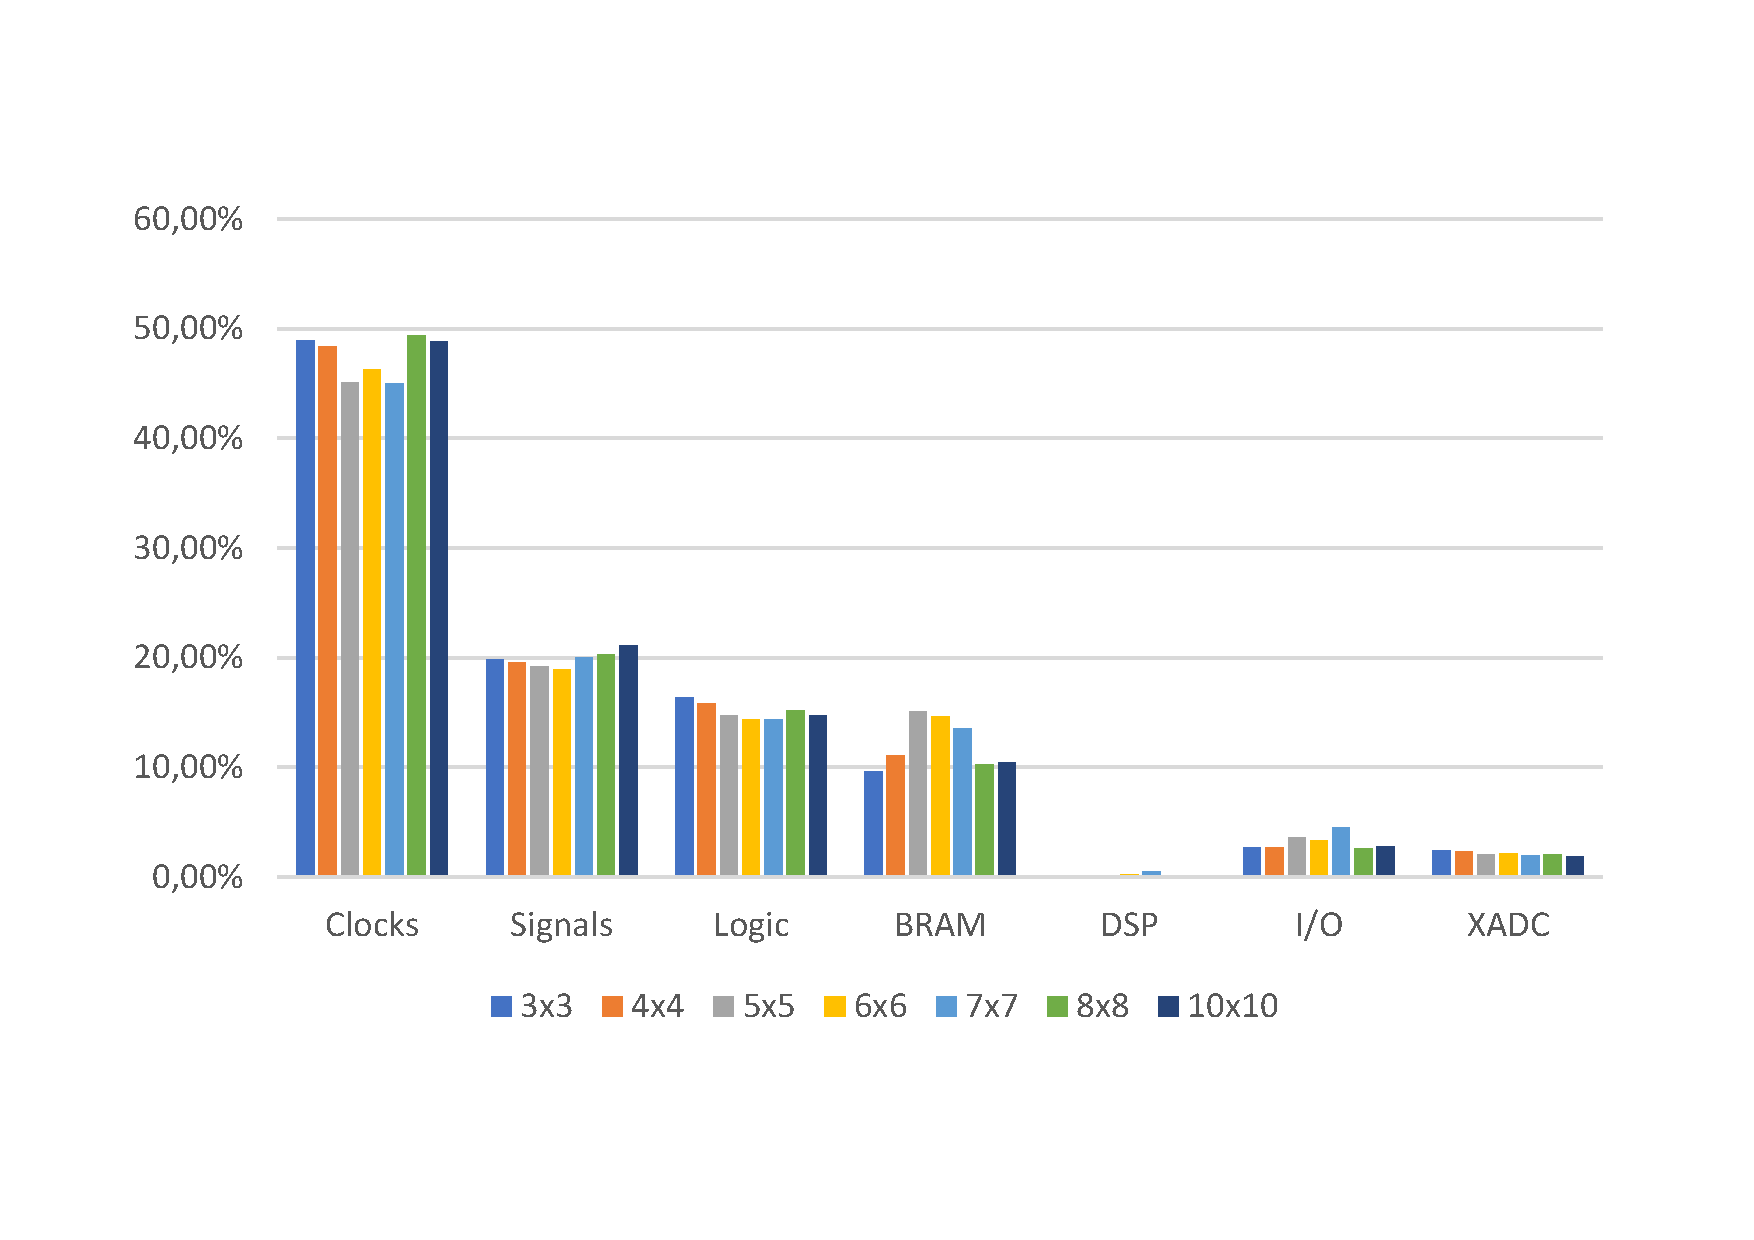
\includegraphics[scale=0.6,angle=0]{./figure/graphs/power_pldyn_div_int16_freq_100mhz.pdf}
\caption{Post Implementation Dynamic Power Consumption per entities in Programmable Logic with a clock frequency of 100 MHz and integer 16 PEs}
\label{fig:dynpowint16ent100}
\end{figure}

\begin{figure}[!htbp]
\centering
\captionsetup{justification=centering}
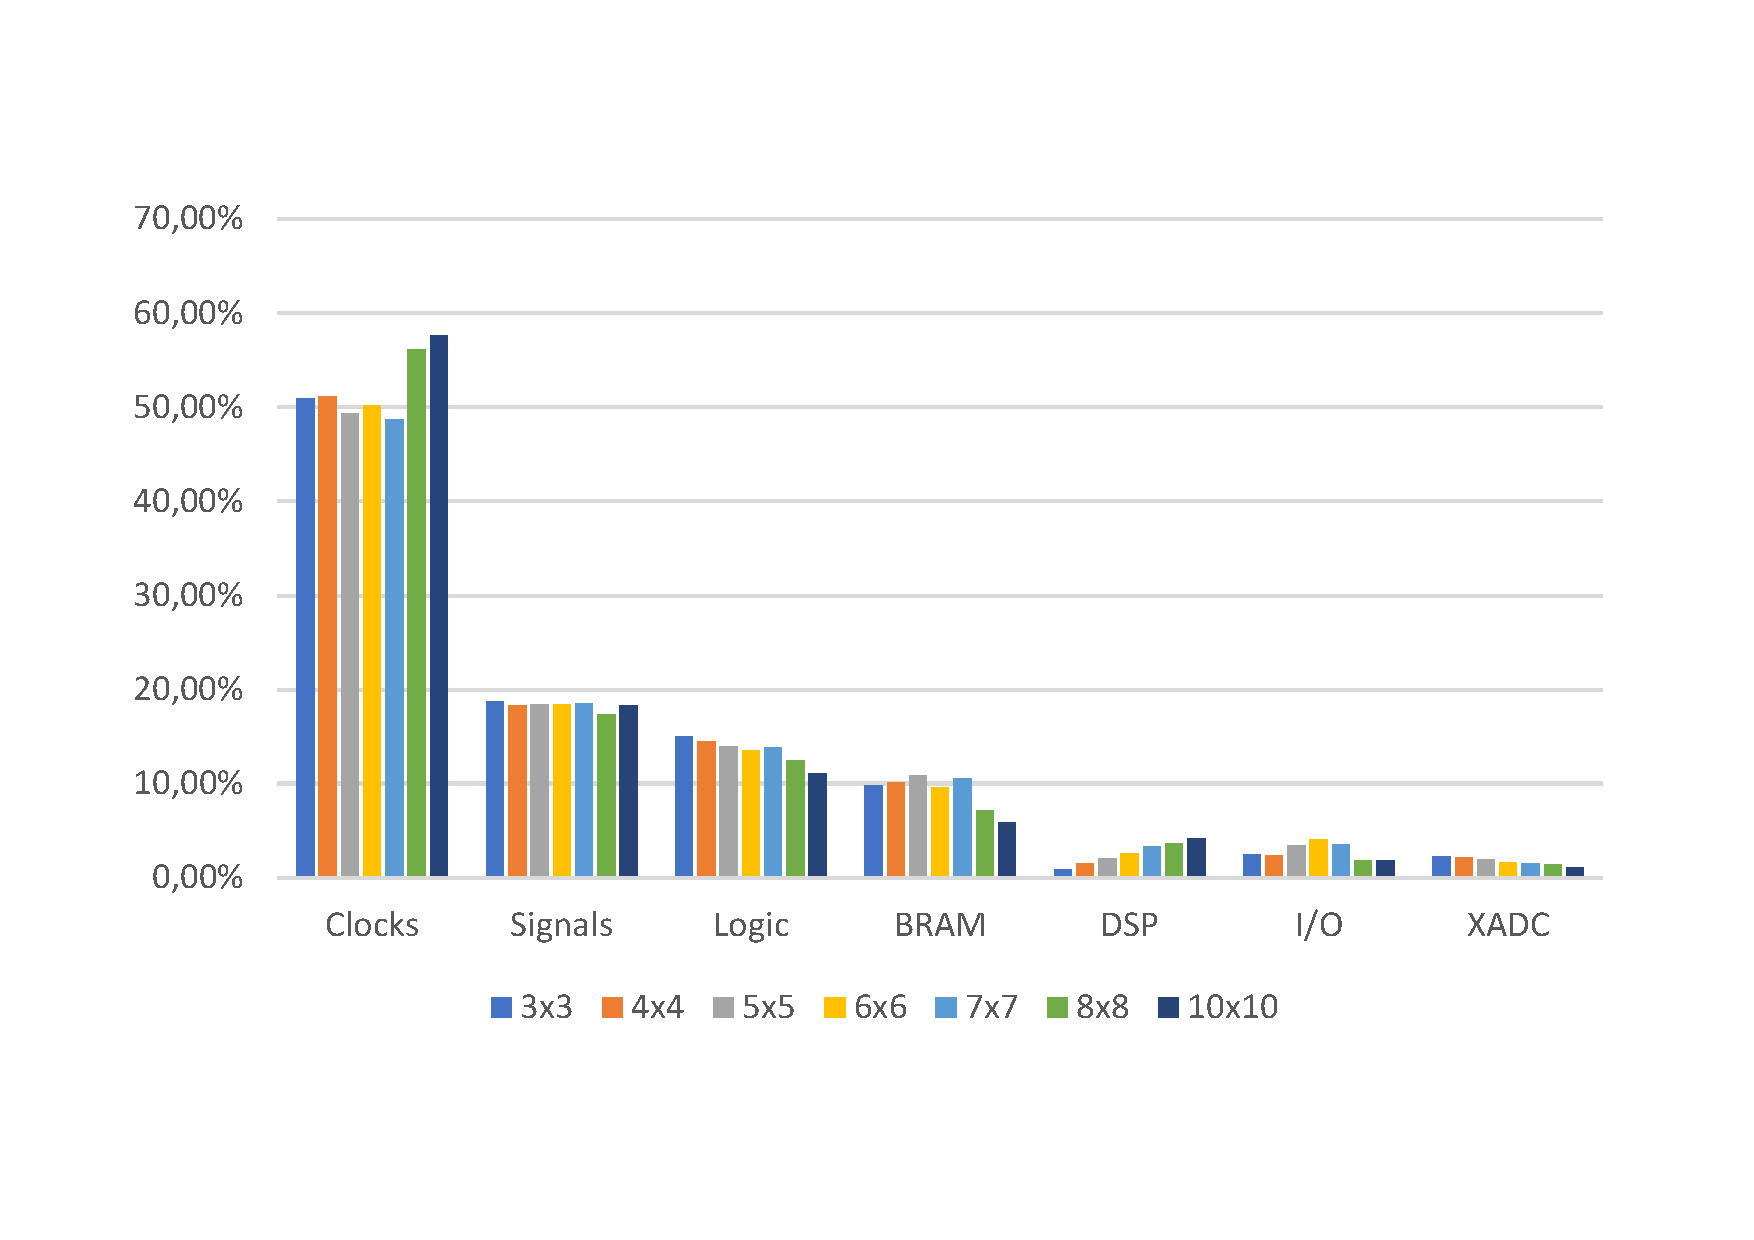
\includegraphics[scale=0.6,angle=0]{./figure/graphs/power_pldyn_div_int32_freq_50mhz.pdf}
\caption{Post Implementation Dynamic Power Consumption per entities in Programmable Logic with a clock frequency of 50 MHz and integer 32 PEs}
\label{fig:dynpowint32ent50}
\end{figure}
\begin{figure}[!htbp]
\centering
\captionsetup{justification=centering}
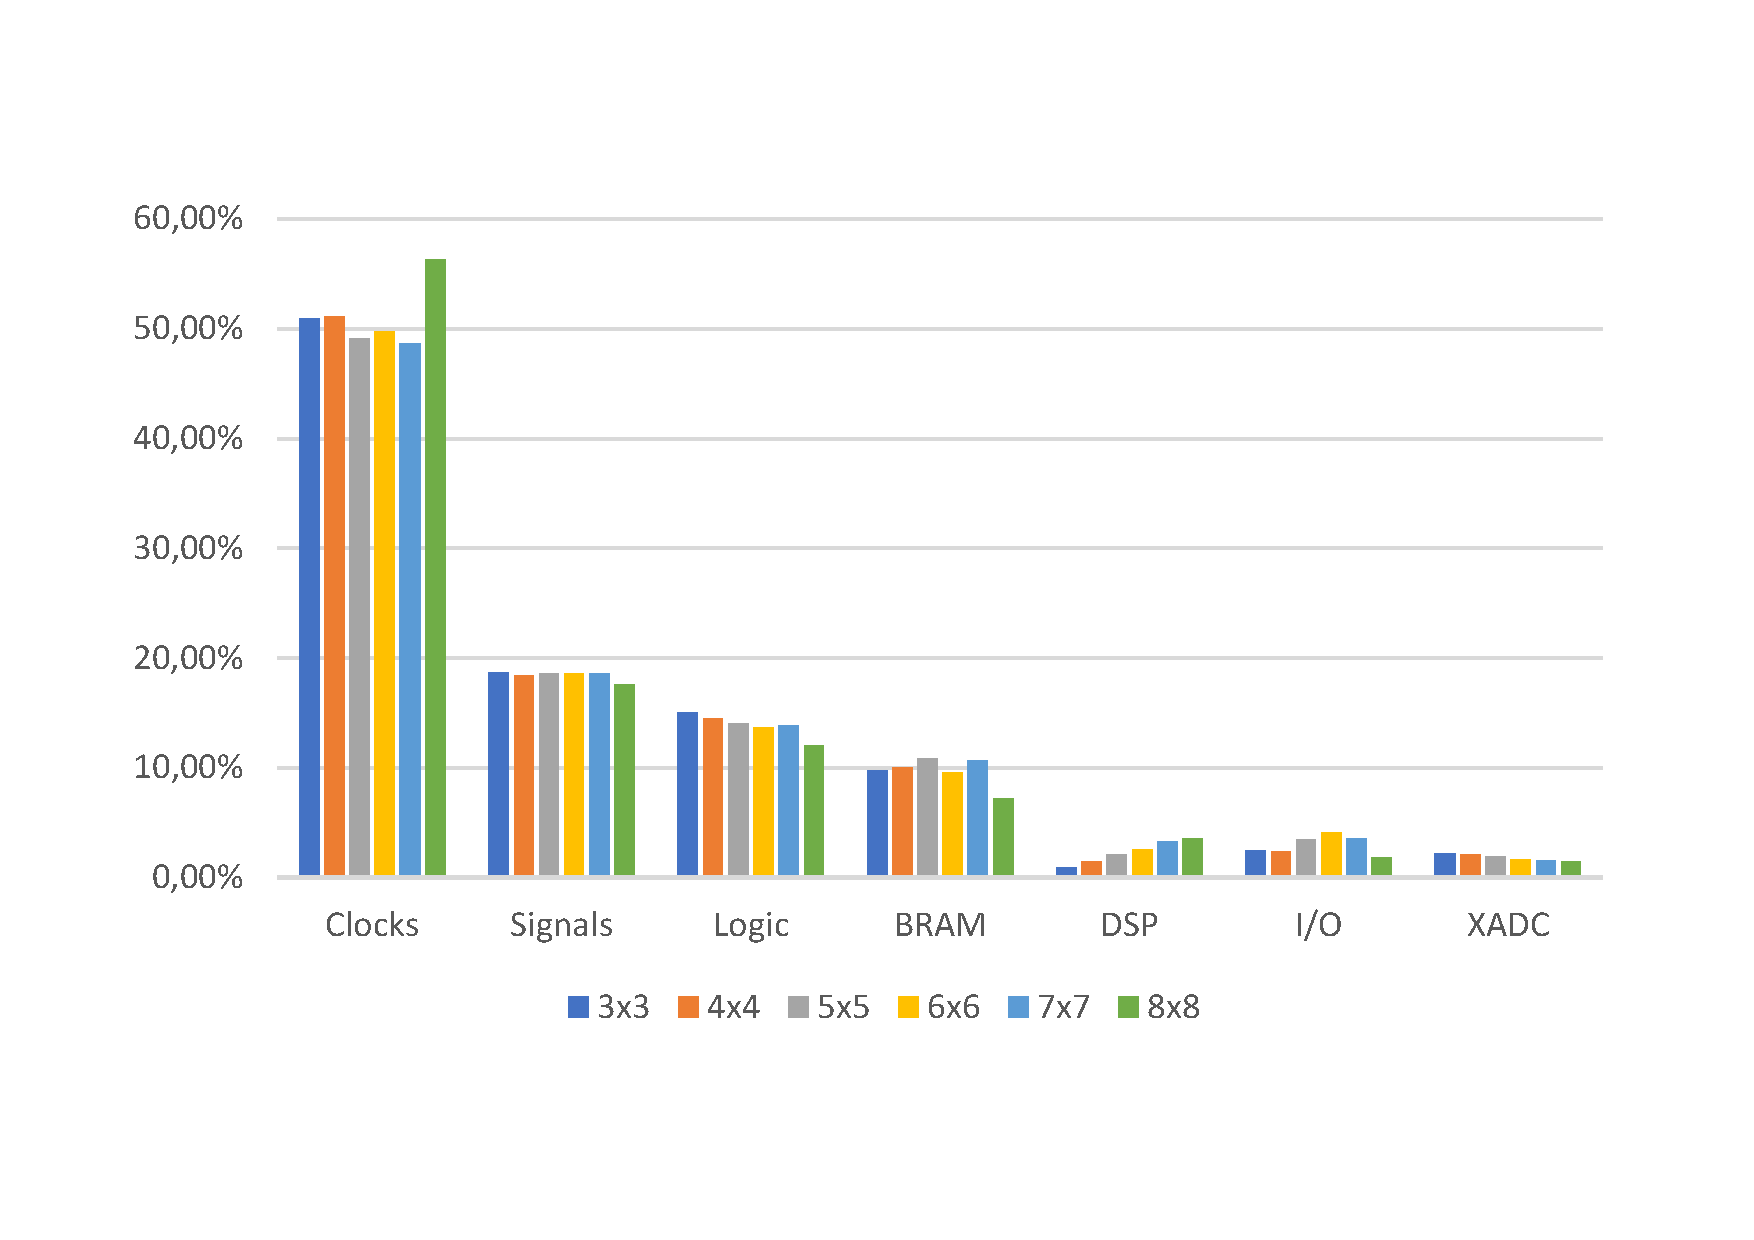
\includegraphics[scale=0.6,angle=0]{./figure/graphs/power_pldyn_div_int32_freq_80mhz.pdf}
\caption{Post Implementation Dynamic Power Consumption per entities in Programmable Logic with a clock frequency of 80 MHz and integer 32 PEs}
\label{fig:dynpowint32ent80}
\end{figure}
\begin{figure}[!htbp]
\centering
\captionsetup{justification=centering}
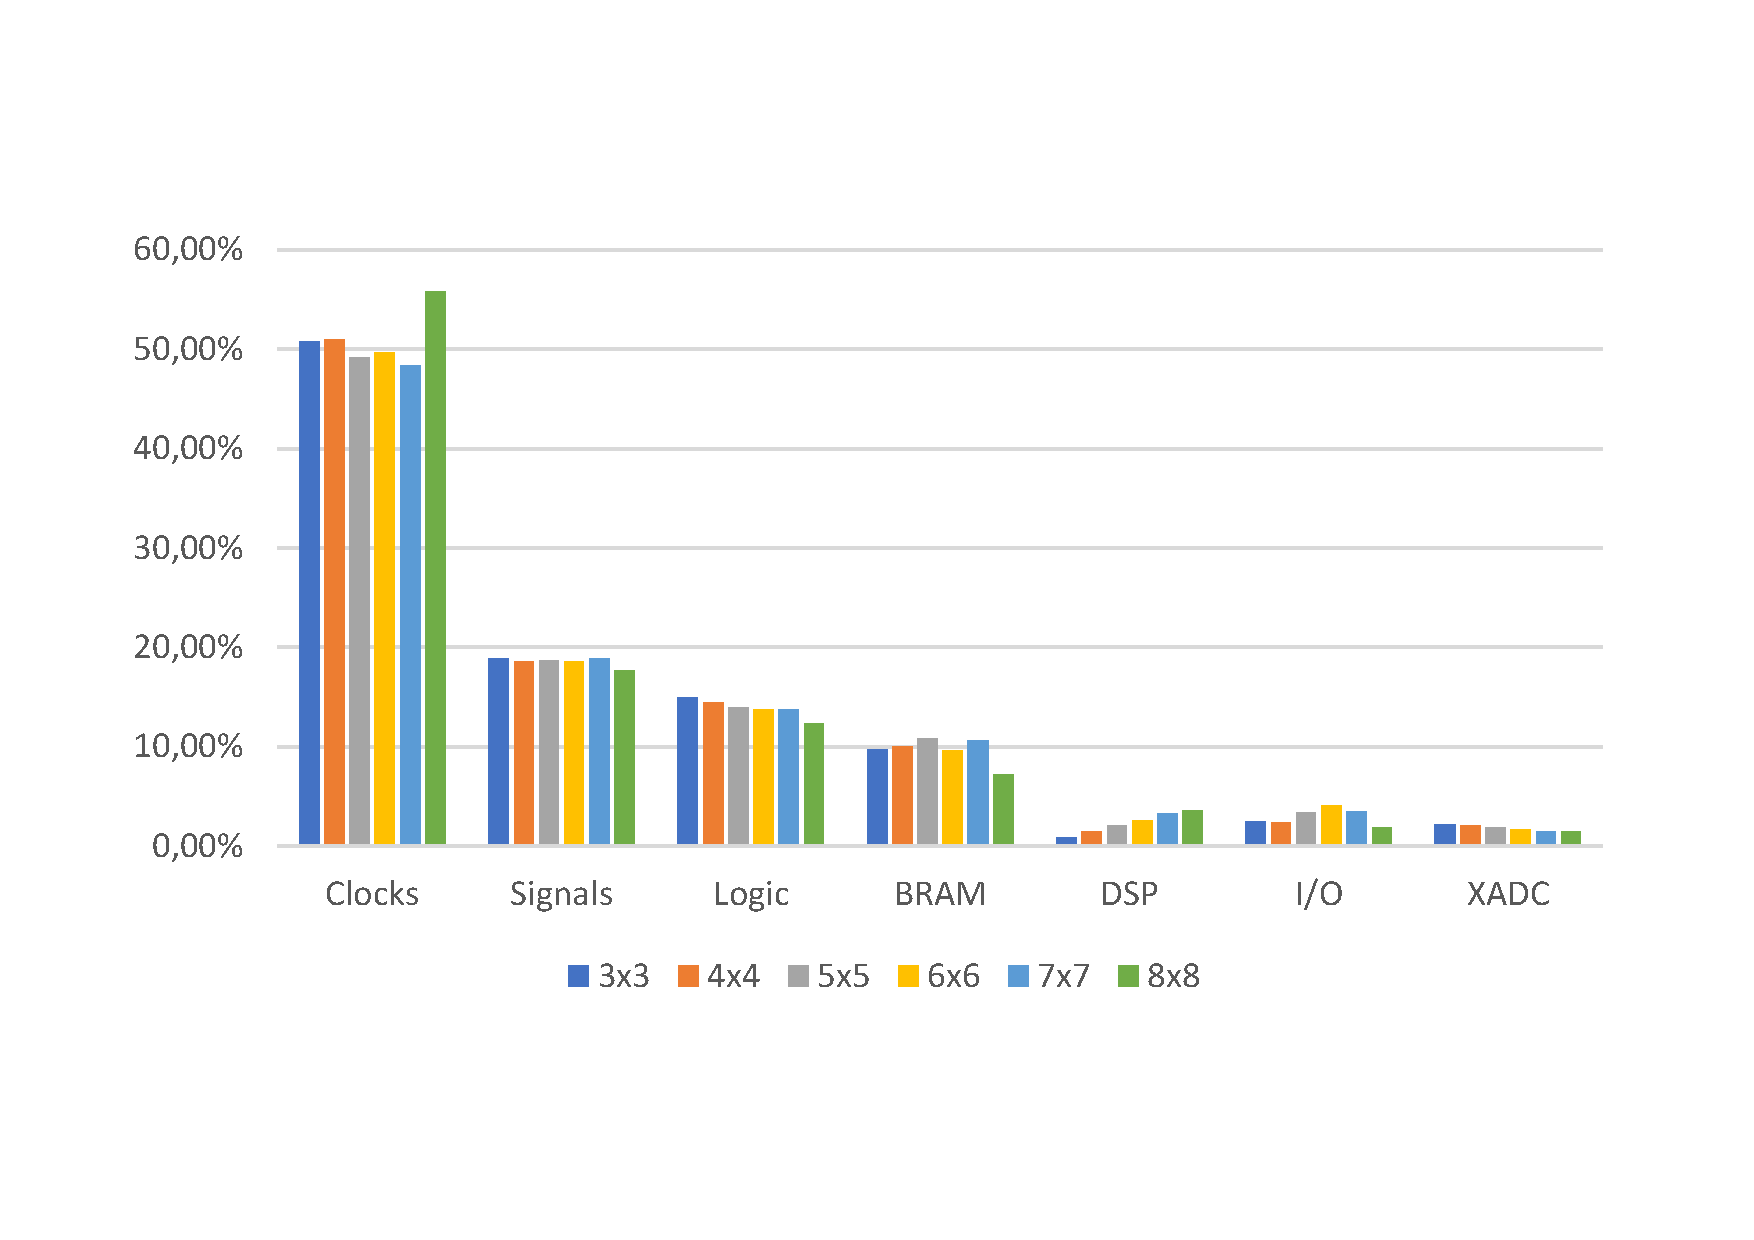
\includegraphics[scale=0.6,angle=0]{./figure/graphs/power_pldyn_div_int32_freq_100mhz.pdf}
\caption{Post Implementation Dynamic Power Consumption per entities in Programmable Logic with a clock frequency of 100 MHz and integer 32 PEs}
\label{fig:dynpowint32ent100}
\end{figure}

\begin{figure}[!htbp]
\centering
\captionsetup{justification=centering}
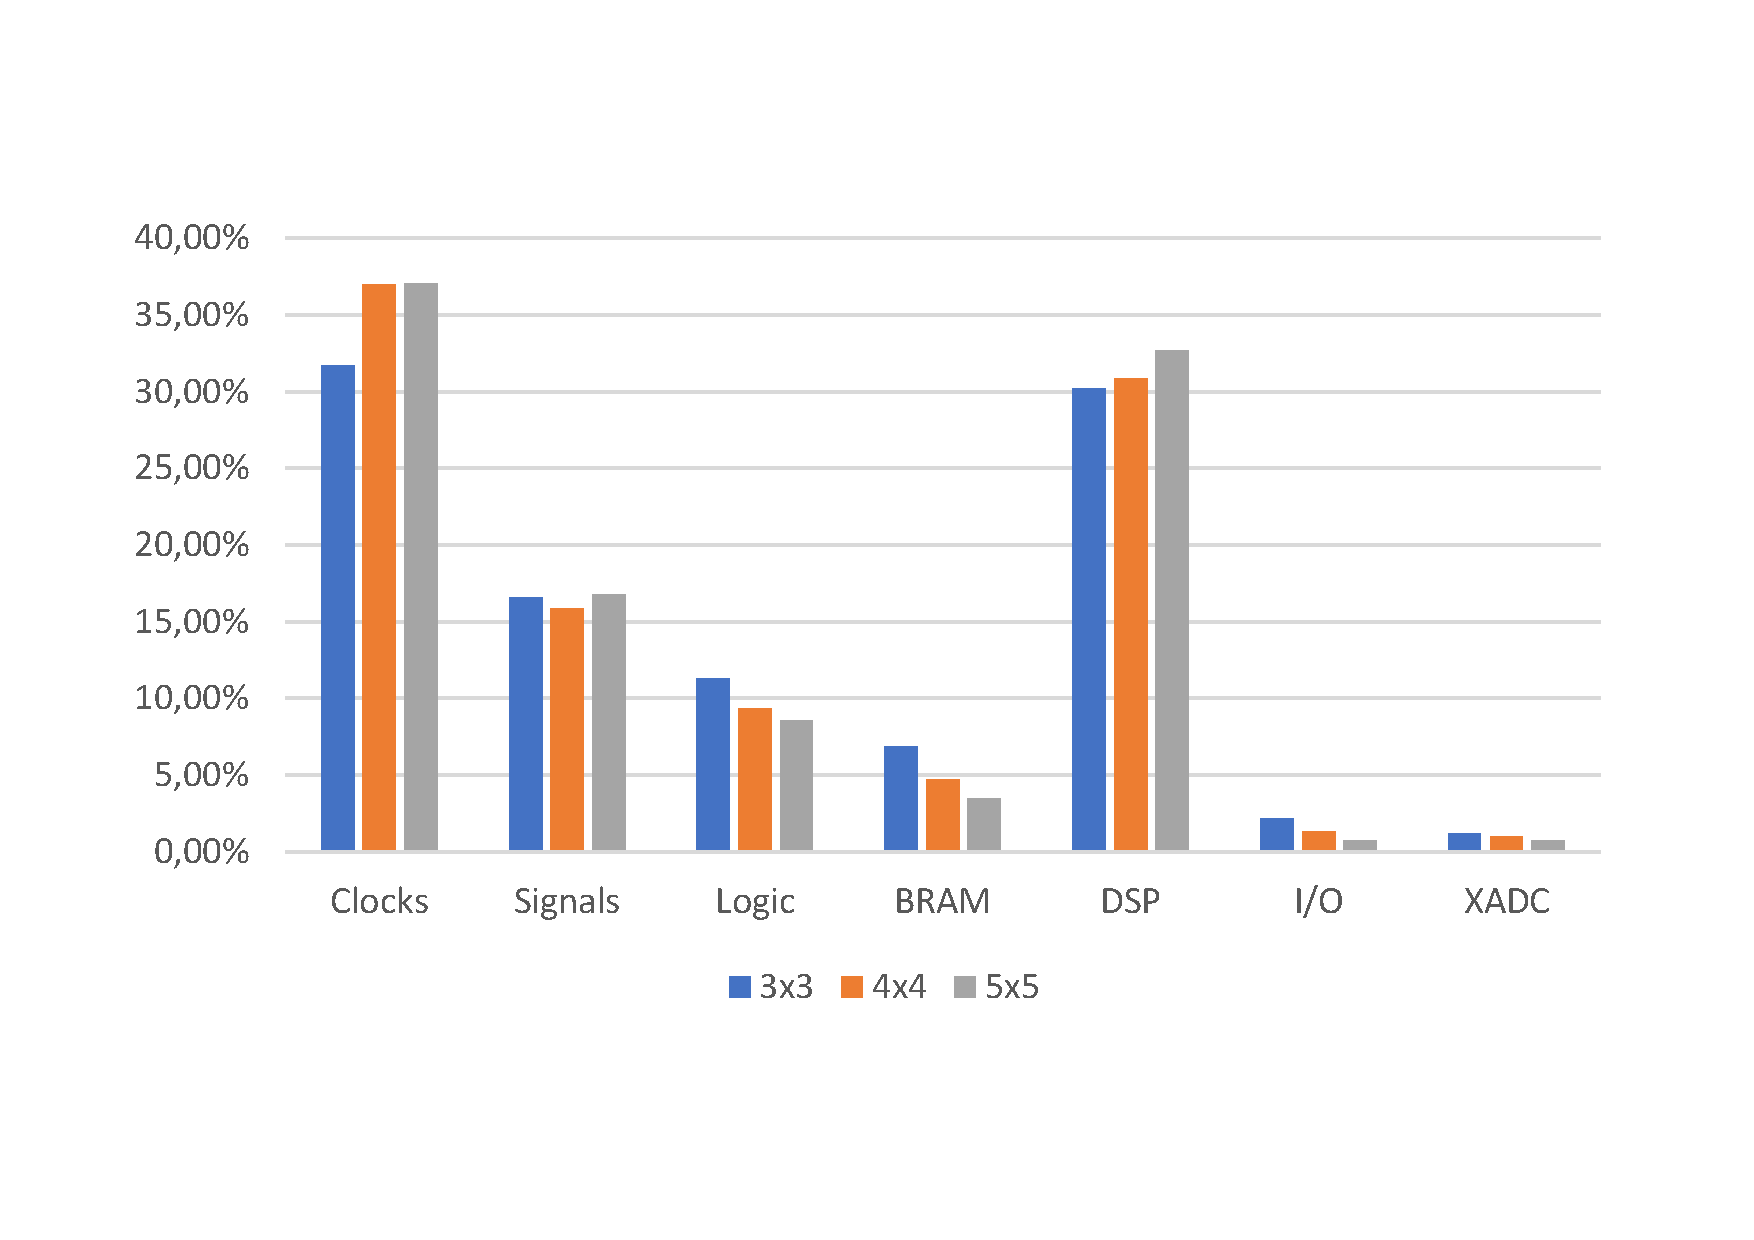
\includegraphics[scale=0.6,angle=0]{./figure/graphs/power_pldyn_div_int64_freq_50mhz.pdf}
\caption{Post Implementation Dynamic Power Consumption per entities in Programmable Logic with a clock frequency of 50 MHz and integer 64 PEs}
\label{fig:dynpowint64ent50}
\end{figure}
\begin{figure}[!htbp]
\centering
\captionsetup{justification=centering}
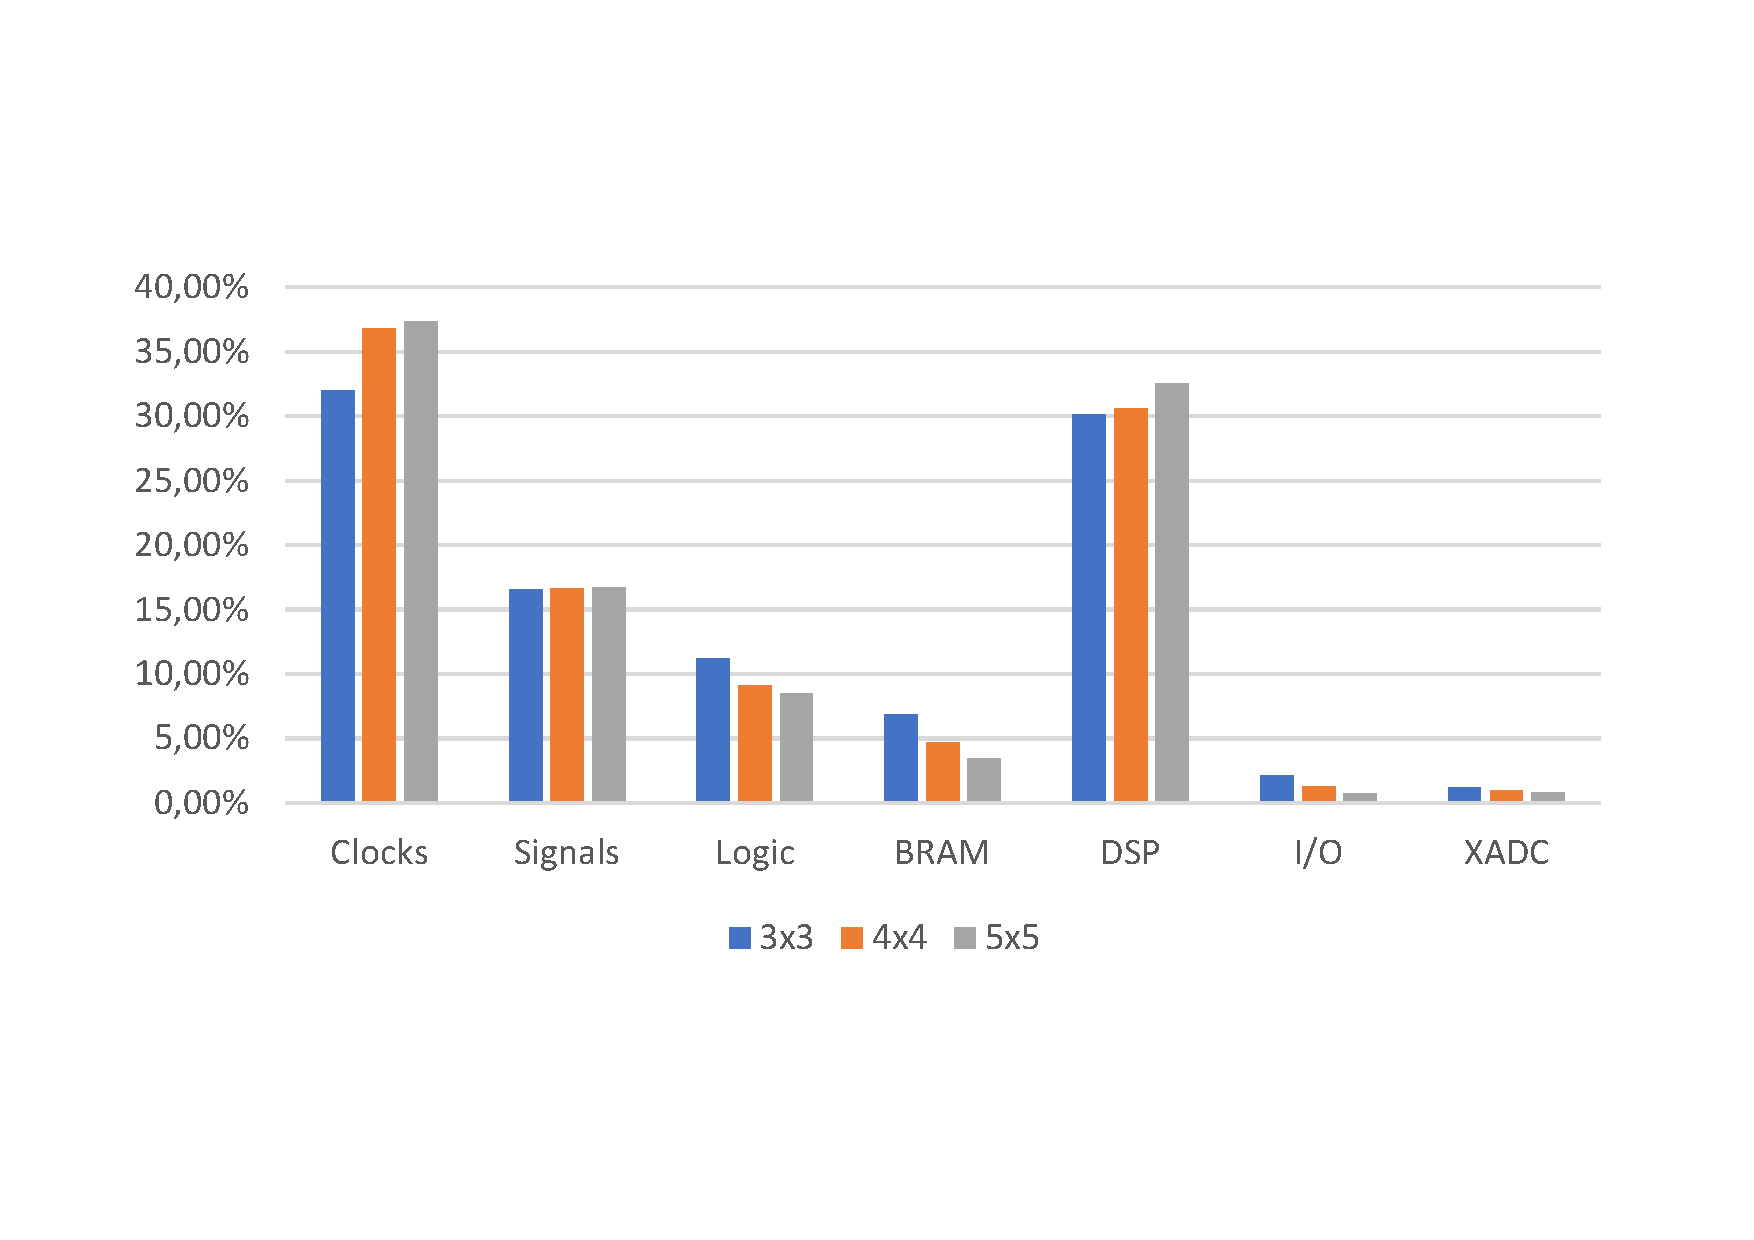
\includegraphics[scale=0.6,angle=0]{./figure/graphs/power_pldyn_div_int64_freq_60mhz.pdf}
\caption{Post Implementation Dynamic Power Consumption per entities in Programmable Logic with a clock frequency of 60 MHz and integer 64 PEs}
\label{fig:dynpowint64ent60}
\end{figure}

